\chapter{Deep Versat}
\label{chapter:DeepVersat}

\quad Versat is a Coarse Grained Reconfigurable Array (CGRA) Architecture. CGRAs are in-between Field Programmable Gate Arrays (FPGA)
 and general purpose processors (GPP).
The former is fully reconfigurable and the highest performance for a workload can be achieved as the Architecture is tailored to the workload.
GPPs on the other hand, are nor reconfigurable and thus slower but are more generic and can process different workloads.
While FPGAs have the granularity at the gate level, CGRAs have the granularity at the functional unit level. They are configurable at run-time and the datapath can be
changed in-between runs.   

In this chapter, the base Versat Architecture will be explained and then the Deep Versat Architecture
 and its improvements.

\section{Versat Architecture}

\quad The Versat Architecture~\cite{sousa:compiler,sousa:controller,sousa:FFT,sousa:versat2016} 
is depicted in figure \ref{figure:oldversat}. Its composed by the following modules: DMA,Controller,Program Memory,Control File Registry,Data-Engine and Configuration module.
The Controller accesses the modules through the control bus. The code made in assembly or C is loaded into the program Memory (RAM) where the user
can write to the configuration module the versat runs. Between runs of the Data Engine,
 the Controller can start doing the next run configuration and calculations.


\begin{figure}[!htbp]
    \centering
    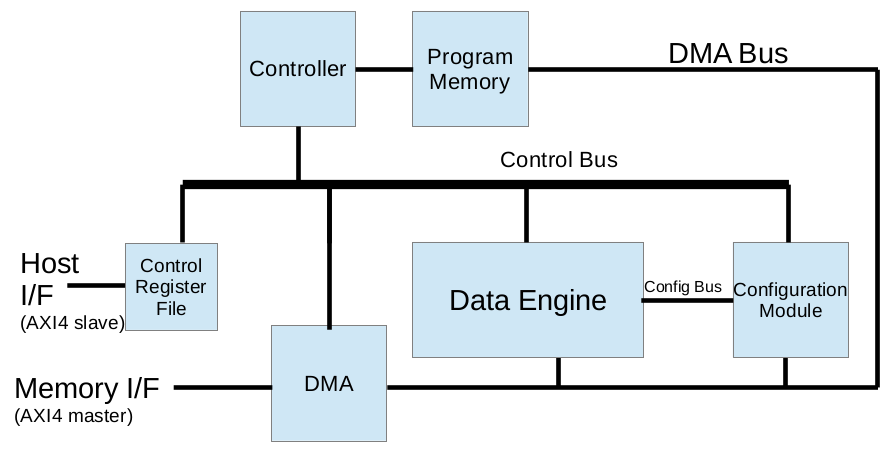
\includegraphics[width=0.8\textwidth]{Figures/top.png}
    \caption{Versat Topology, taken from~\cite{sousa:controller}}
    \label{figure:oldversat}
\end{figure} 

\subsection{Data Engine}
\quad The Data Engine which is represented in figure \ref{figure:DE} carries out the computation needed on the data arrays. Its a 32 bit Architecture with up to 11 Functional Units:
 Arithmetic and Logic Unit(ALU), stripped down ALU (ALU-Lite),
 Multiplier and Accumulator (MAC) and Barrel Shifter.
 Depending on the project and calculations, a new type of FU or the existing ones can be altered to support the algorithm.
 The DE has a full mesh  topology, that means that each FU can be the output to another, This decreases the operating frequency.

 Each Input of a Functional Unit has a Mux with 19 entries, 8 of which are from the memories (2 from each Mem out of 4 total units) and the rest from the Functional Units (11).

 \begin{figure}[!htbp]
    \centering
    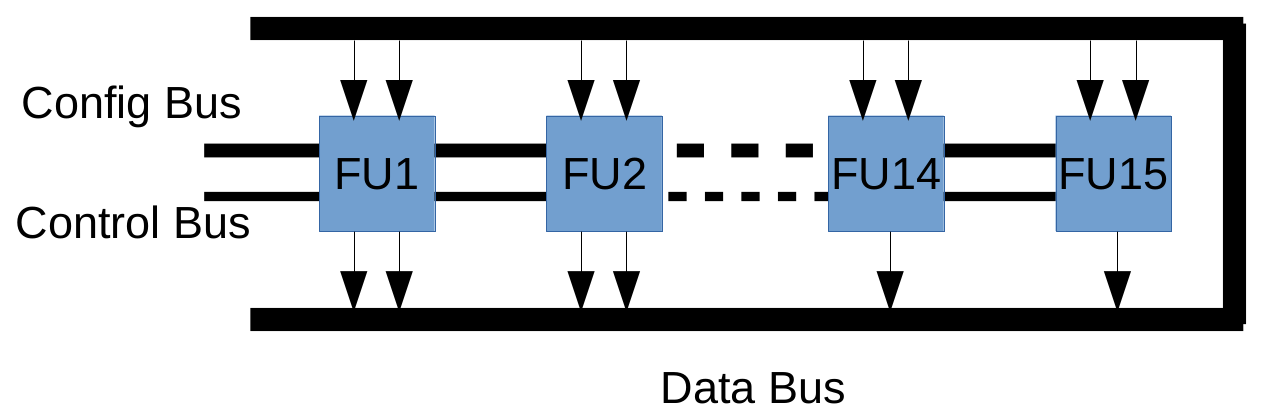
\includegraphics[width=1\textwidth]{Figures/de.png}
    \caption{Versat Data Engine Topology, taken from~\cite{sousa:FFT}}
    \label{figure:DE}
\end{figure} 

 The 4 Memories are dual port and for the input of both ports, 
 there is an Address Generation Unit (AGU) that is able to 
 reproduce two nested loops of memory indexes.
 The AGUs control which MEM data is the input of the FUs and where
 to store the results of the operation. Also, the AGUs support a delayed start to line up timings
due to latencies.

\begin{figure}[!htbp]
    \centering
    \includegraphics[width=0.8\textwidth]{Figures/fu.pdf}
    \caption{Versat Functional Unit, taken from~\cite{lopes:versat}}
    \label{figure:FU}
\end{figure} 


\newpage
\subsection{Configuration Module}
\quad Versat has several configuration spaces devised for each Functional Unit,
with each space having multiple fields to define the operation of the Functional unit (e.g which op for the ALU).
These are accessed before the run by the controller to define the datapath.

\begin{figure}[!htbp]
    \centering
    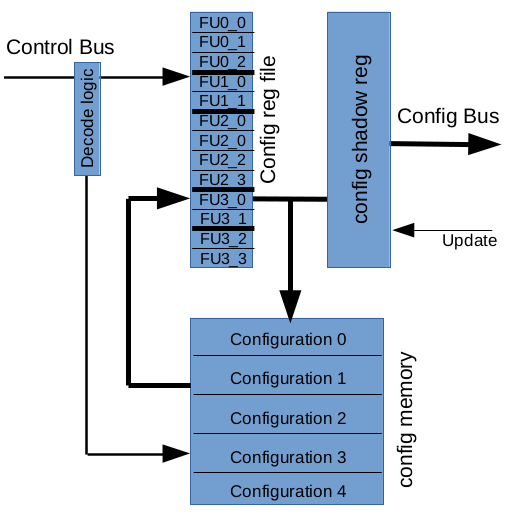
\includegraphics[width=0.6\textwidth]{Figures/conf.png}
    \caption{Configuration Module,taken from~\cite{sousa:controller}}
    \label{figure:conf}
\end{figure} 

The Configuration Module (CM), depicted in figure \ref{figure:conf}, 
has three components:configuration memory, variable length configuration register file 
and configuration shadow register.
The latter holds the current configuration so the controller can change the values of the configuration file in-between runs.
The decode logic finds which component to write or read, if its the registers, it ignores read operations.
Meanwhile, the configuration memory interprets both write and reads. When it receives a read,
it writes into the register configuration data, when its a write, it stores the data instead.


\newpage
\section{Deep Versat Architecture}


\begin{figure}[!htb]
    \centering
    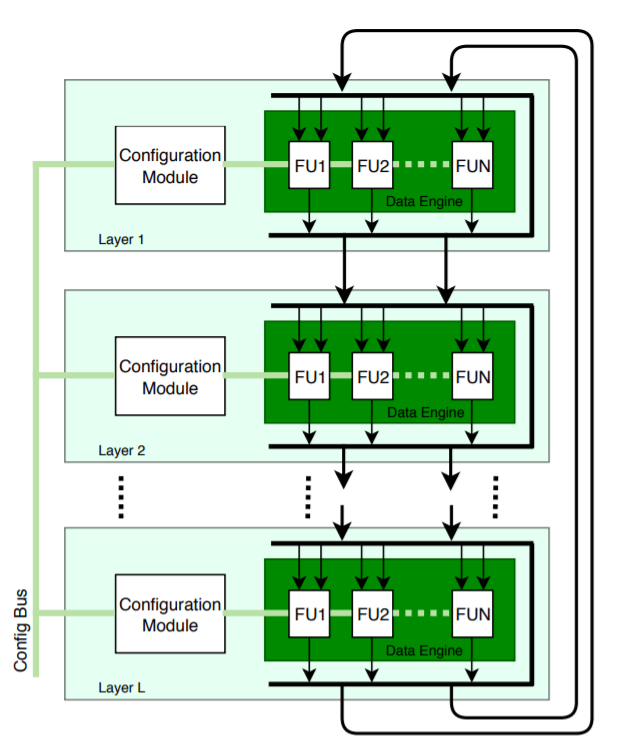
\includegraphics[width=0.7\textwidth]{Figures/deep-versat.png}
    \caption{Deep Versat Architecture, taken from~\cite{valter:deepversat}}
    \label{figure:deepversatarch}
\end{figure} 

\quad The Deep Versat Architecture\cite{valter:deepversat}
, in figure \ref{figure:deepversatarch}, decouples the Data Engine (DE) from all control and as such, it can be used with any CPU. 
It can be paired with hard cores in
FPGA boards like the ZYNC board %cite here
with its A9 ARM dual core CPUs or pair it with a soft core.

Its principle is to create the concept of a Versat Core: Configuration Module (CM) and its Functional Units (FU) connected with a control bus and a data bus.
Instead of writing to a memory, there is the option to write for the next
Versat Core to create more complex and more complete Datapaths, to avoid
having to reconfigure a lot of times.

The number of Layers and FUs are reconfigurable pre-silicon with the only limitation
that each layer is identical. To program Deep Versat, an API is generated
from the Verilog .vh files. 




\newpage
\subsection{Deep Versat System}

\begin{figure}[!htbp]
    \centering
    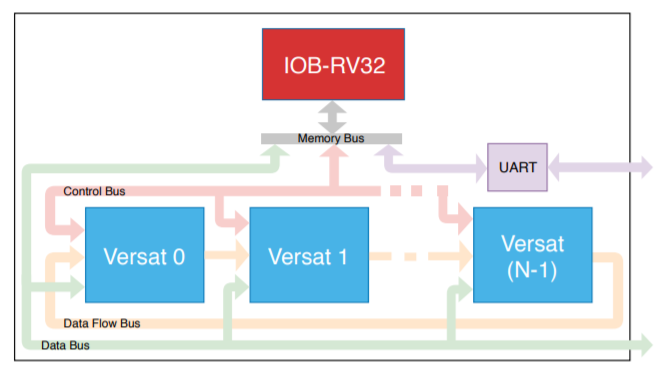
\includegraphics[width=0.8\textwidth]{Figures/deep-versat-top.png}
    \caption{Deep Versat System, taken from~\cite{valter:deepversat}}
    \label{figure:deepversattop}
\end{figure} 

\quad To make a complete system, a new controller is needed with a more robust toolchain.
In a recent dissertation~\cite{valter:deepversat}, the IOB-RV32 processor was used which uses the RISC-V 32IM. The core is derived from
the open source PicoRV32 CPU~\cite{picorv}.
The IOB-RV32 uses its memory bus to access peripherals in which Deep Versat and the UART module are connected as such.
The control bus is used to access the configuration modules of Deep Versat. The data bus is used to read and write
large amount of data into Deep Versat. The data flow bus is reserved for inter Versat Core communication.

\begin{table}[!htbp]
    \centering
    \begin{tabular}{|ll|}
        \hline
        \textbf{Peripheral}     & \textbf{Memory address} \\ \hline
        UART module             & 12’h100xxxxx            \\ \hline
        Deep Versat control bus & 8’h11xxxxxx             \\ \hline
        Deep Versat data bus    & 8’h12xxxxxx             \\ \hline
        \end{tabular}
    \caption{Deep Versat Memory Map}
    \label{table:deepversat}
    \end{table}


The memory map to address the peripherals,
 including deep versat, is in table \ref{table:deepversat}.
 Each Versat has 15 bits of address while the CPU addresses
 the peripherals with 32 bits, with 8 of those occupied to chose
 the peripheral in question. That leaves 9 bits to address several Versat Cores
 which brings the theoretical maximum versat cores to 512. The IOB-RV32 is compatible with the
 GNU toolchain to offer better portability of code and alongside the C++ Versat API the difficulty
 to code for the System diminishes.
